%%%%%%%%%%%%%%%%%%%%%%%%%%%%%%%%%%%%%%%%%%%%%%%%%%%%%%%%%%%%%%%%%%%%%%%%%%%%%%%%%%%%%%%%%%%%
%%
%% Chapter 3 : Related works
%%
%%      * Should give an overview of what the big dogs are saying in the field
%%
%%  BASIC STRUCTURE :
%%
%%      a. DeepRL algorithms
%%          * Natural Policy Gradients
%%          * Trust region policy optimization
%%          * Proximal Policy Optimization
%%
%%      b. DeepRL and robot locomotion
%%          * Benchmarking drl for continuous ccontrol (2016?)
%%          * DeepTerrainRL
%%          * DeepLoco
%%          * DeepMimic
%%          * Emergence of locomotion in rich and complex environments
%%
%%      c. Current benchmarks for robot locomotion
%%          * DeepMind's ControlSuite
%%          * OpenAI's mujoco-py
%%          * Berkeley's garage and rllab
%%          * Stanford's robosuite
%%          * NVIDIA Isaac + FleX
%%          * UBC's terrainRlSim
%%          * Unity's ml-agents (talk about the marathon envs)
%%
%%
%%%%%%%%%%%%%%%%%%%%%%%%%%%%%%%%%%%%%%%%%%%%%%%%%%%%%%%%%%%%%%%%%%%%%%%%%%%%%%%%%%%%%%%%%%%%


\chapter{Related Works}
\label{ch:relatedWorks}

%%%%%%%%%%%%%%%%%%%%%%%%%%%%%%%
%   Figures for chapter 3 - 
%%%%%%%%%%%%%%%%%%%%%%%%%%%%%%%

%% \newcommand{\figFrameworkFlow}{
%%     \begin{figure}
%%         \centering
%%         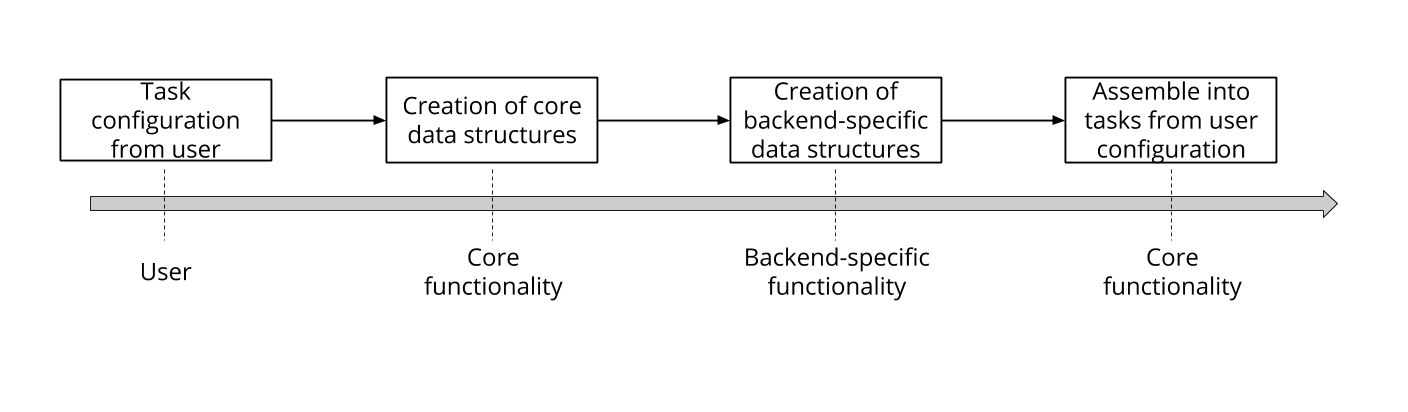
\includegraphics[width=0.9\textwidth]{./chapters/chapter_4/imgs/img_ch4_framework_flow.png}
%%         \caption{Flow of data in the proposed framework}
%%         \label{fig:ch4_proposed_framework_flow}
%%     \end{figure}
%% }

%% \newcommand{\figFrameworkCoreSensor}{
%%     \begin{figure}[!ht]
%%         \centering
%%         \begin{subfigure}[b]{0.3\textwidth}
%%             \centering
%%             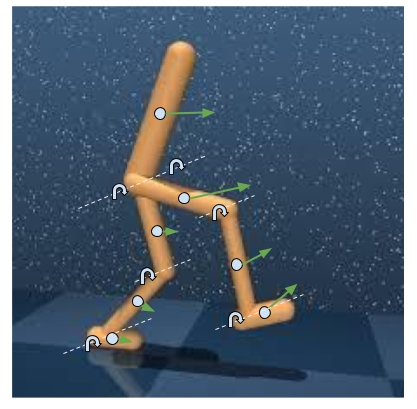
\includegraphics[width=0.9\textwidth]{./chapters/chapter_4/imgs/img_ch4_sensors_core_1.png}
%%             \caption{}
%%             \label{fig:ch4_core_sensor_1}
%%         \end{subfigure}
%%         \begin{subfigure}[b]{0.3\textwidth}
%%             \centering
%%             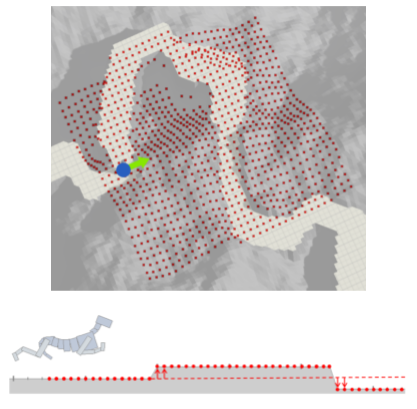
\includegraphics[width=0.9\textwidth]{./chapters/chapter_4/imgs/img_ch4_sensors_core_2.png}
%%             \caption{}
%%             \label{fig:ch4_core_sensor_2}
%%         \end{subfigure}
%%         \begin{subfigure}[b]{0.3\textwidth}
%%             \centering
%%             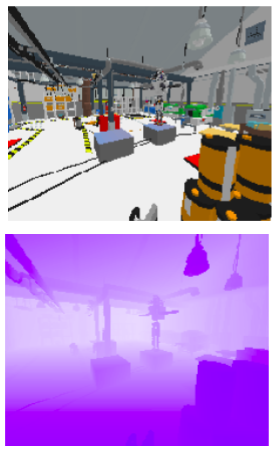
\includegraphics[width=0.9\textwidth]{./chapters/chapter_4/imgs/img_ch4_sensors_core_3.png}
%%             \caption{}
%%             \label{fig:ch4_core_sensor_3}
%%         \end{subfigure}
%%         \caption{Core sensors functionality. a) Intrinsic readings from joints and bodies (adapted from [@CITE]).
%%                                              b) Extrinsic readings from heightmaps of the terrain (adapted from [@CITE,@CITE]).
%%                                              c) Extrinsic readings from rgb and depth images of the agent view (adapted from [@CITE]).}
%%         \label{fig:ch4_core_sensor_functionality}
%%     \end{figure}
%% }

\newcommand{\figPolicyChanges}{
    \begin{figure}[!ht]
        \centering
        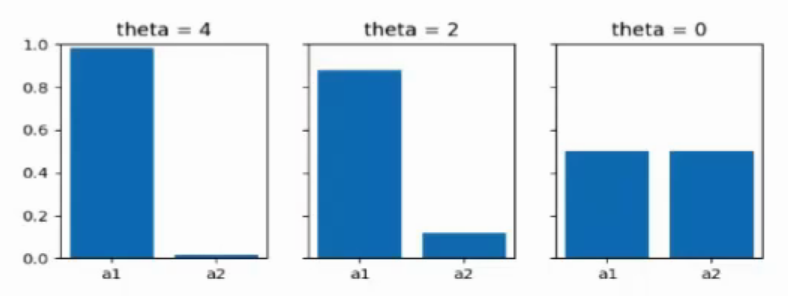
\includegraphics[width=0.8\textwidth]{./chapters/chapter_3/imgs/img_ch3_euclidean_constraint.png}
        \caption{A simple example that shows that same changes in parameter space yield 
                 very different changes in policy space. Adapted from \href{https://youtu.be/yqYKeWtUSO8?t=1050}{this} lecture.}
        \label{fig:ch3_policy_changes}
    \end{figure}
}

\newcommand{\figBenchmarkControlSuite}{
	\begin{figure}
		\centering
		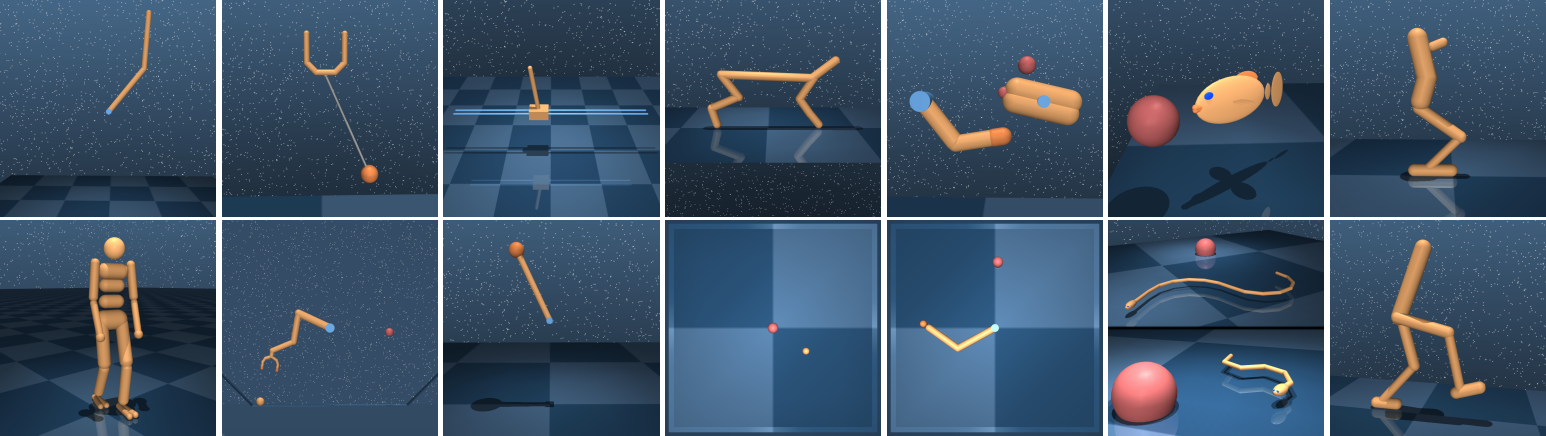
\includegraphics[width=0.9\textwidth]{./chapters/chapter_3/imgs/img_ch3_controlsuite.png}
		\caption{Models available in the Controlsuite benchmark. 
				 Extracted from \citet{Controlsuite}}
	    \label{fig:ch3_controlsuite}
	\end{figure}
}

\newcommand{\figBenchmarkOpenAIGymMujoco}{
    \begin{figure}[!ht]
        \centering
        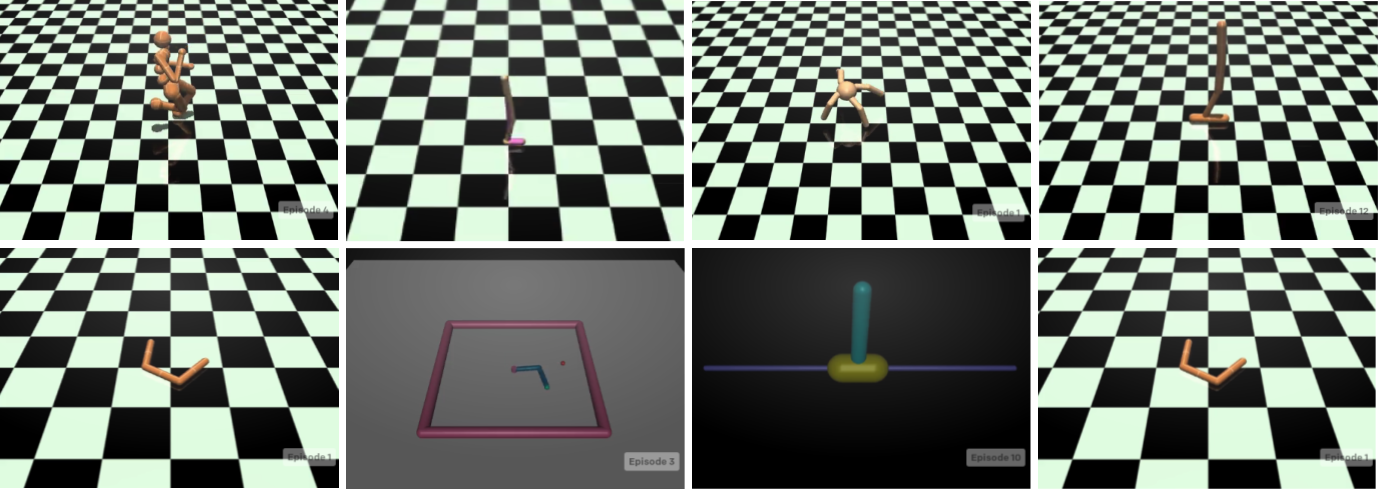
\includegraphics[width=0.9\textwidth]{./chapters/chapter_3/imgs/img_ch3_openaigym_mujoco.png}
        \caption{Models available in the OpenAI-gym benchmark with mujoco as backend. 
                 Extracted from \citet{Gym}}
        \label{fig:ch3_openaigym_mujoco}
    \end{figure}
}

\newcommand{\figBenchmarkOpenAIGymRoboschool}{
    \begin{figure}[!ht]
        \centering
        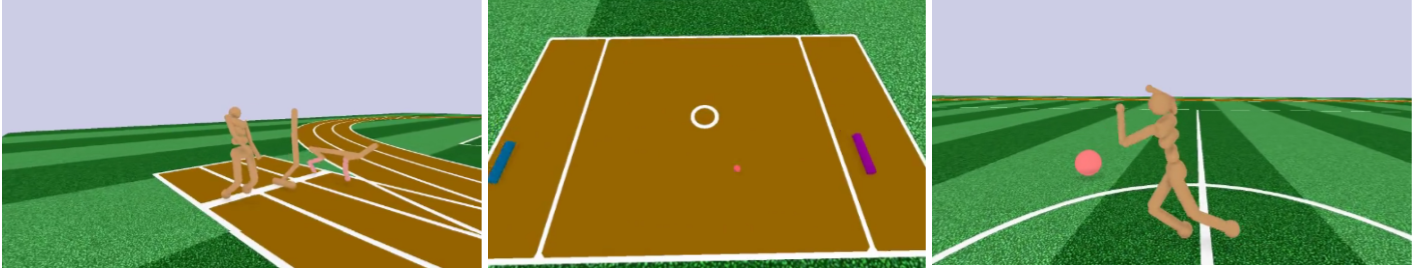
\includegraphics[width=1.0\textwidth]{./chapters/chapter_3/imgs/img_ch3_openaigym_roboschool.png}
        \caption{Models available in the OpenAI-gym benchmark with Bullet as backend. 
                 Extracted from \citet{Roboschool}}
        \label{fig:ch3_openaigym_roboschool}
    \end{figure}
}

\newcommand{\figBenchmarkRllabClassic}{
    \begin{figure}[!ht]
        \centering
        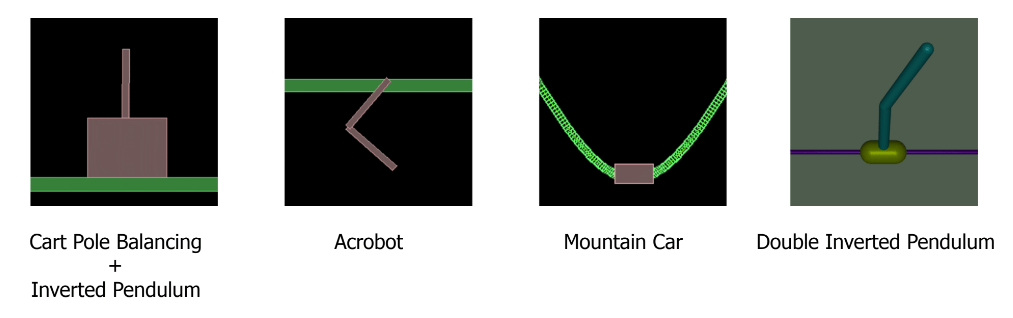
\includegraphics[width=0.9\textwidth]{./chapters/chapter_3/imgs/img_ch3_rllab_classic.png}
        \caption{Models available in the Rllab classic benchmark. Extracted from \cite{Rllab}}
        \label{fig:ch3_rllab_classic}
    \end{figure}
}

\newcommand{\figBenchmarkRllabLocomotion}{
    \begin{figure}[!ht]
        \centering
        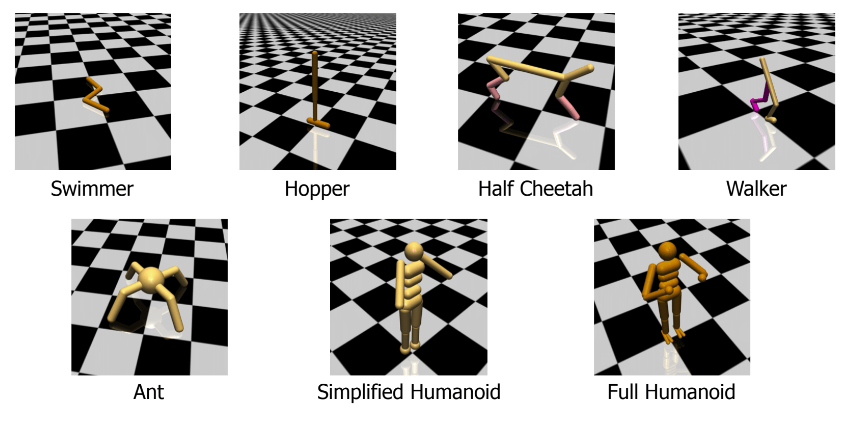
\includegraphics[width=0.9\textwidth]{./chapters/chapter_3/imgs/img_ch3_rllab_locomotion.png}
        \caption{Models available in the Rllab locomotion benchmark. Extracted from \citet{Rllab}}
        \label{fig:ch3_rllab_locomotion}
    \end{figure}
}

\newcommand{\figBenchmarkRllabHierarchical}{
    \begin{figure}[!ht]
        \centering
        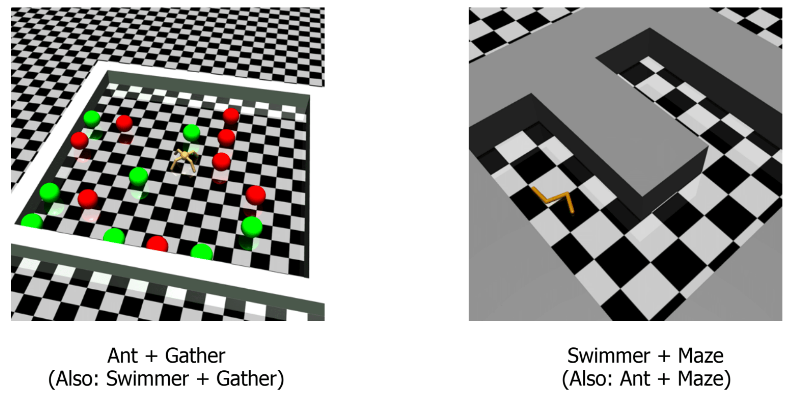
\includegraphics[width=0.9\textwidth]{./chapters/chapter_3/imgs/img_ch3_rllab_hierarchical.png}
        \caption{Models available in the Rllab hierarchical benchmark. Extracted from \citet{Rllab}}
        \label{fig:ch3_rllab_hierarchical}
    \end{figure}
}

\newcommand{\figBenchmarksRobosuite}{
    \begin{figure}[!ht]
        \centering
        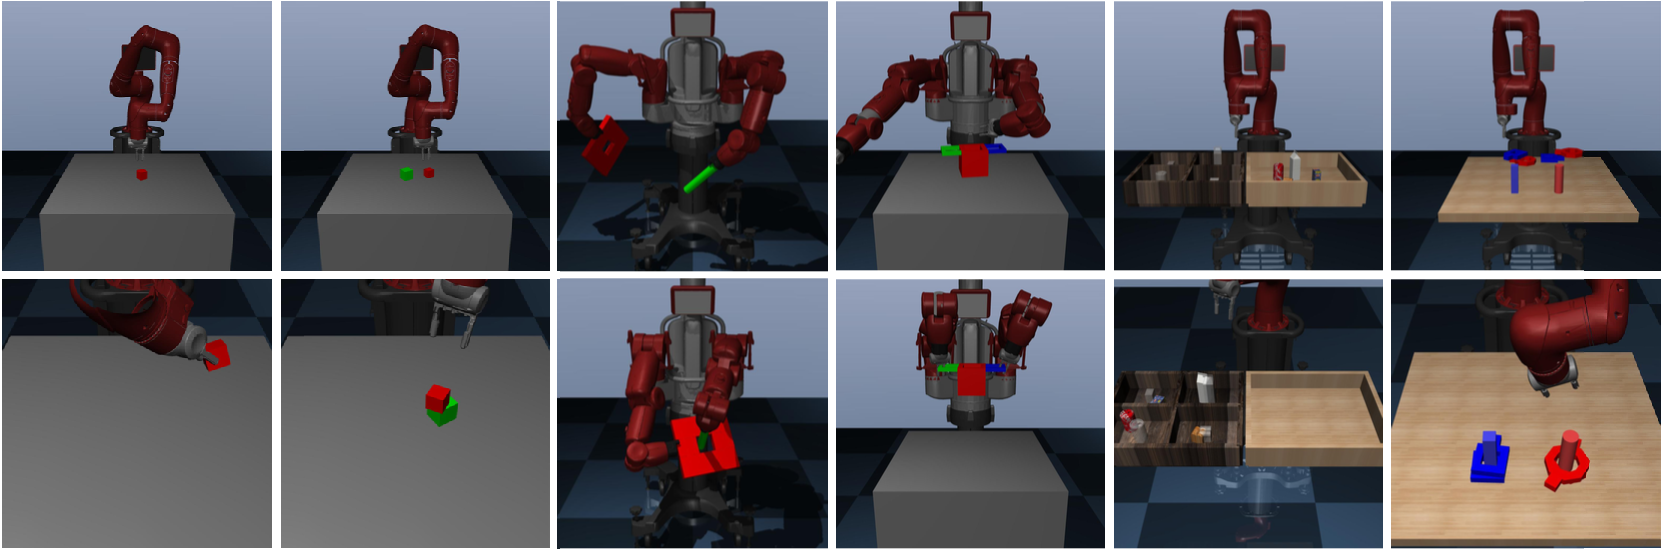
\includegraphics[width=1.0\textwidth]{./chapters/chapter_3/imgs/img_ch3_robosuite.png}
        \caption{Tasks available in Robosuite, as part of the Surreal framework \citep{Surreal}}
        \label{fig:ch3_robosuite}
    \end{figure}
}

\newcommand{\figBenchmarksGpuSim}{
    \begin{figure}[!ht]
        \centering
        \begin{subfigure}[b]{0.3\textwidth}
            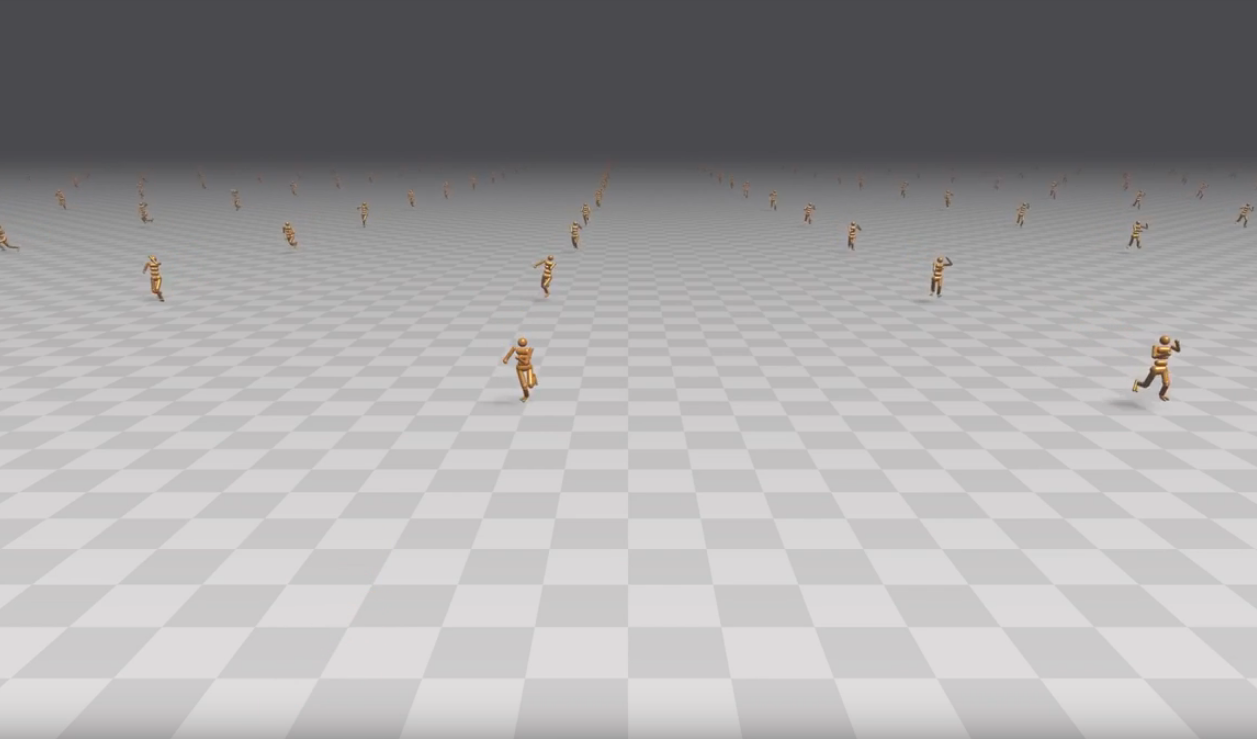
\includegraphics[width=1.0\textwidth]{./chapters/chapter_3/imgs/img_ch3_gpu_sim_1.png}
        \end{subfigure}
        \begin{subfigure}[b]{0.3\textwidth}
            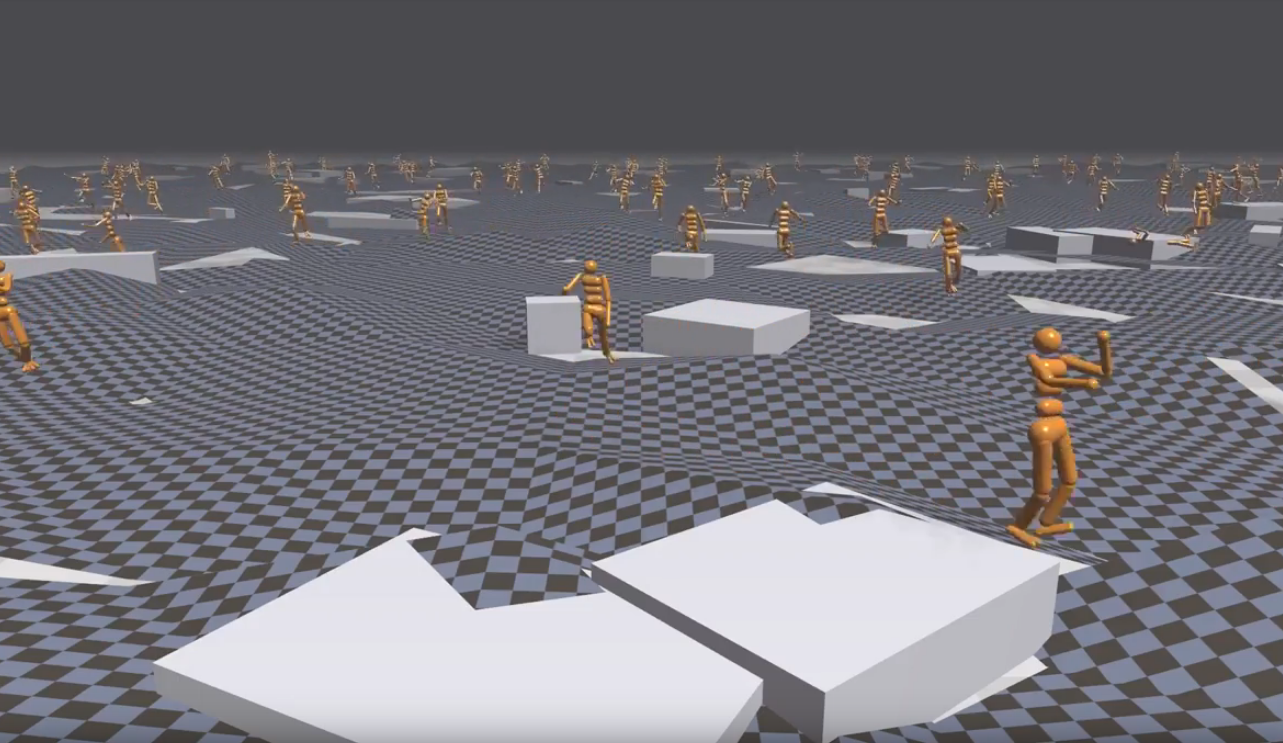
\includegraphics[width=1.0\textwidth]{./chapters/chapter_3/imgs/img_ch3_gpu_sim_2.png}
        \end{subfigure}
        \begin{subfigure}[b]{0.3\textwidth}
            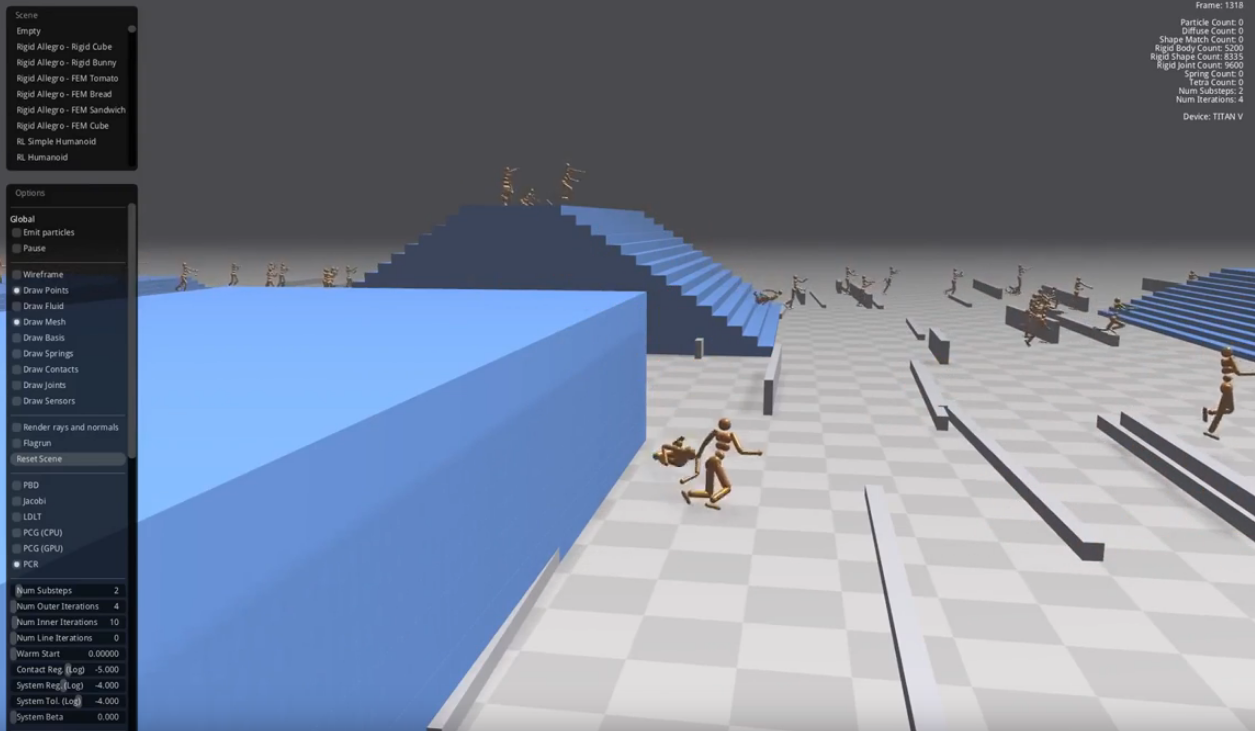
\includegraphics[width=1.0\textwidth]{./chapters/chapter_3/imgs/img_ch3_gpu_sim_3.png}
        \end{subfigure}
        \caption{Tasks provided in the Gpu-Accelerated simulator by \citep{GpuSim}}
        \label{fig:ch3_gpusim}
    \end{figure}
}

\newcommand{\figBenchmarksTerrainRLSim}{
    \begin{figure}[!ht]
        \centering
        \begin{subfigure}[b]{0.3\textwidth}
            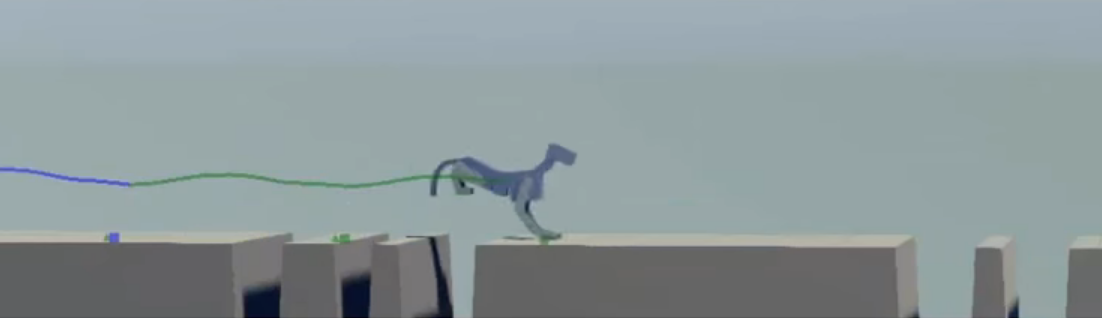
\includegraphics[width=1.0\textwidth]{./chapters/chapter_3/imgs/img_ch3_terrainrlsim_1.png}
            \caption{}
        \end{subfigure}
        \begin{subfigure}[b]{0.3\textwidth}
            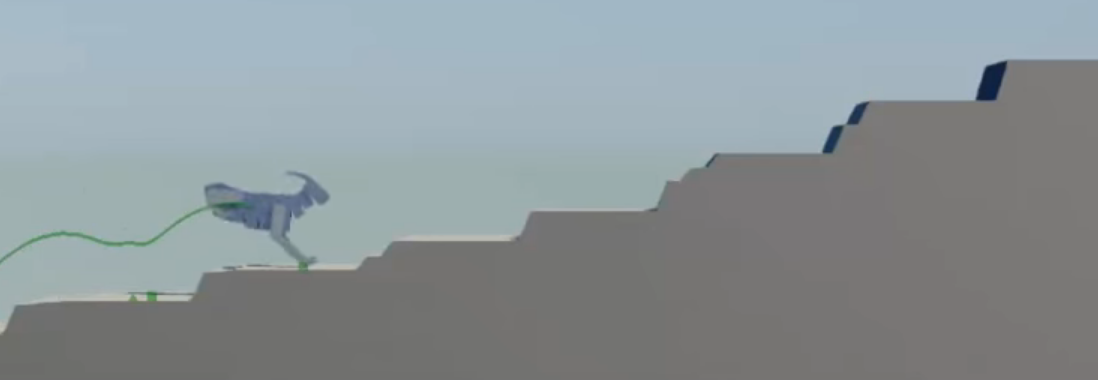
\includegraphics[width=1.0\textwidth]{./chapters/chapter_3/imgs/img_ch3_terrainrlsim_2.png}
            \caption{}
        \end{subfigure}
        \begin{subfigure}[b]{0.3\textwidth}
            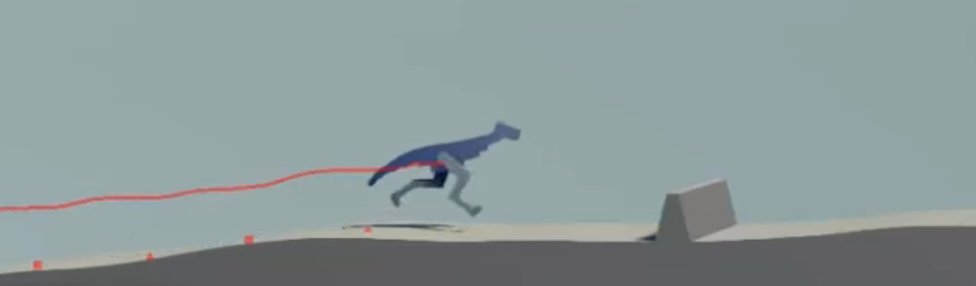
\includegraphics[width=1.0\textwidth]{./chapters/chapter_3/imgs/img_ch3_terrainrlsim_3.png}
            \caption{}
        \end{subfigure}

        \centering
        \begin{subfigure}[b]{0.3\textwidth}
            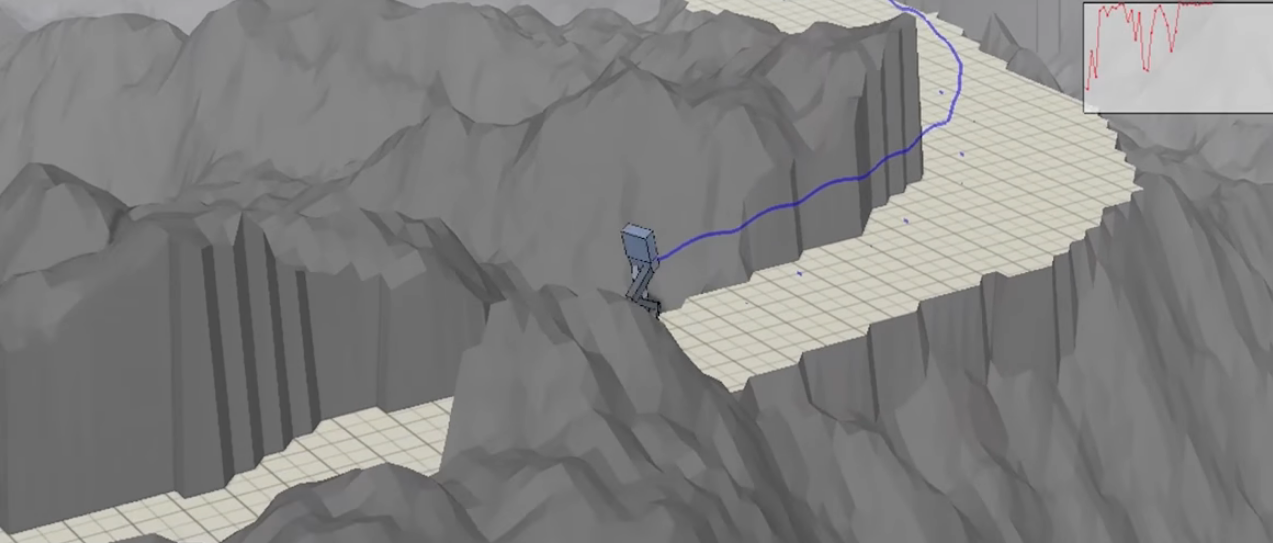
\includegraphics[width=1.0\textwidth]{./chapters/chapter_3/imgs/img_ch3_terrainrlsim_4.png}
            \caption{}
        \end{subfigure}
        \begin{subfigure}[b]{0.3\textwidth}
            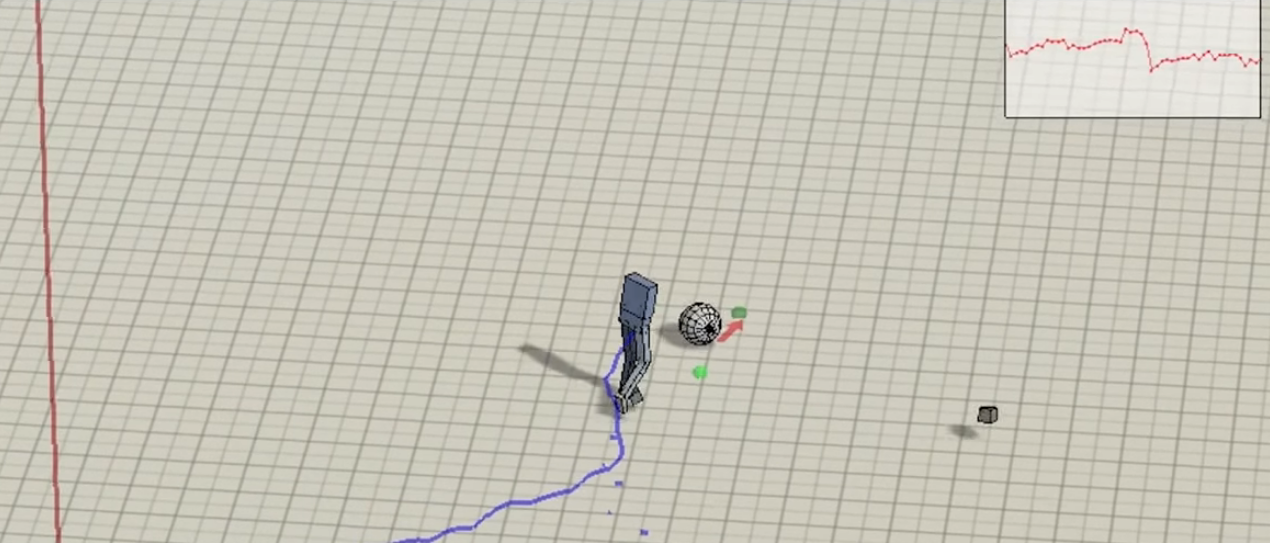
\includegraphics[width=1.0\textwidth]{./chapters/chapter_3/imgs/img_ch3_terrainrlsim_5.png}
            \caption{}
        \end{subfigure}
        \begin{subfigure}[b]{0.3\textwidth}
            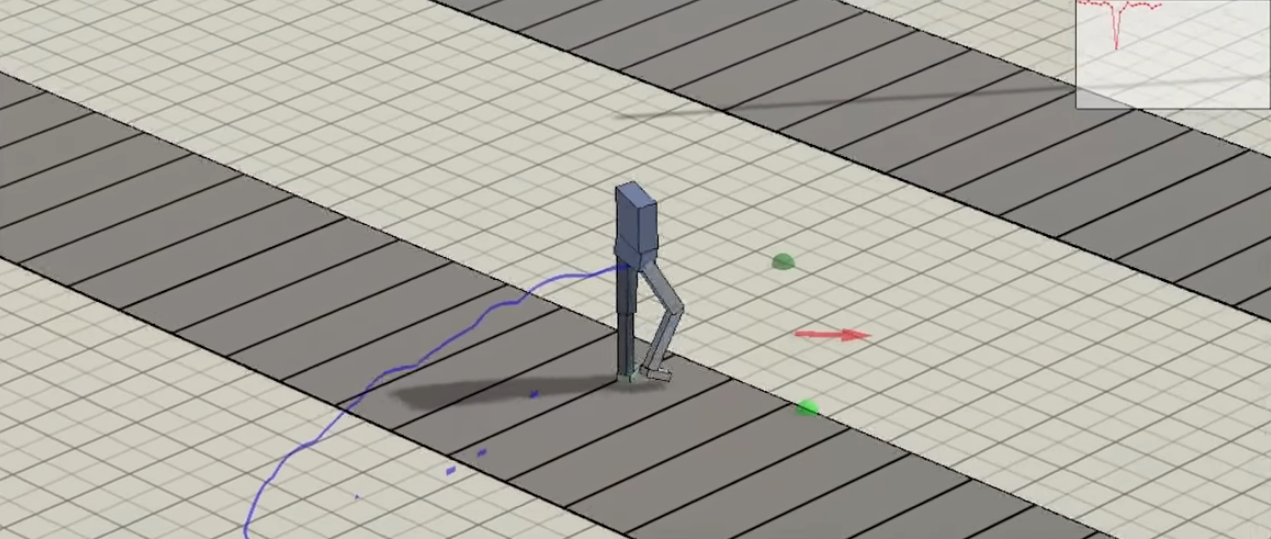
\includegraphics[width=1.0\textwidth]{./chapters/chapter_3/imgs/img_ch3_terrainrlsim_6.png}
            \caption{}
        \end{subfigure}

        \centering
        \begin{subfigure}[b]{0.3\textwidth}
            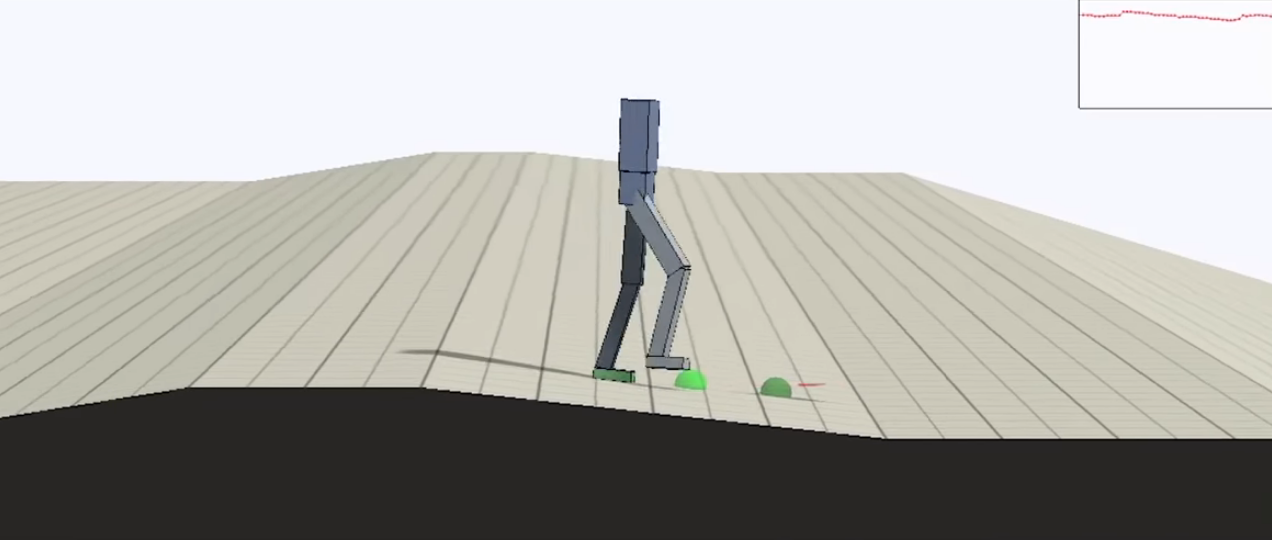
\includegraphics[width=1.0\textwidth]{./chapters/chapter_3/imgs/img_ch3_terrainrlsim_7.png}
            \caption{}
        \end{subfigure}
        \begin{subfigure}[b]{0.3\textwidth}
            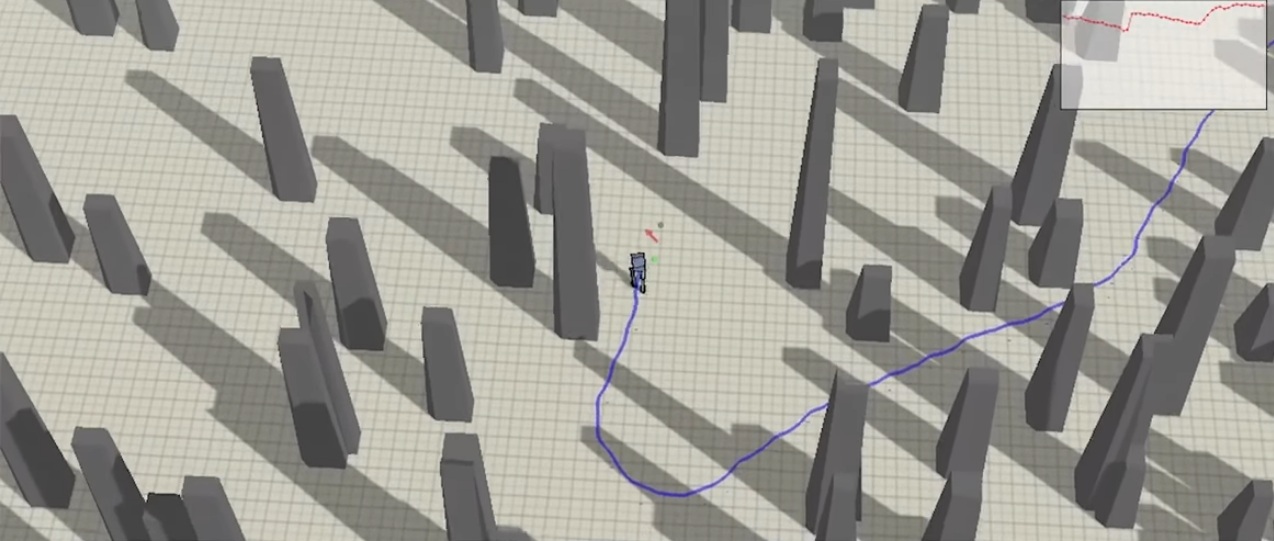
\includegraphics[width=1.0\textwidth]{./chapters/chapter_3/imgs/img_ch3_terrainrlsim_8.png}
            \caption{}
        \end{subfigure}
        \begin{subfigure}[b]{0.3\textwidth}
            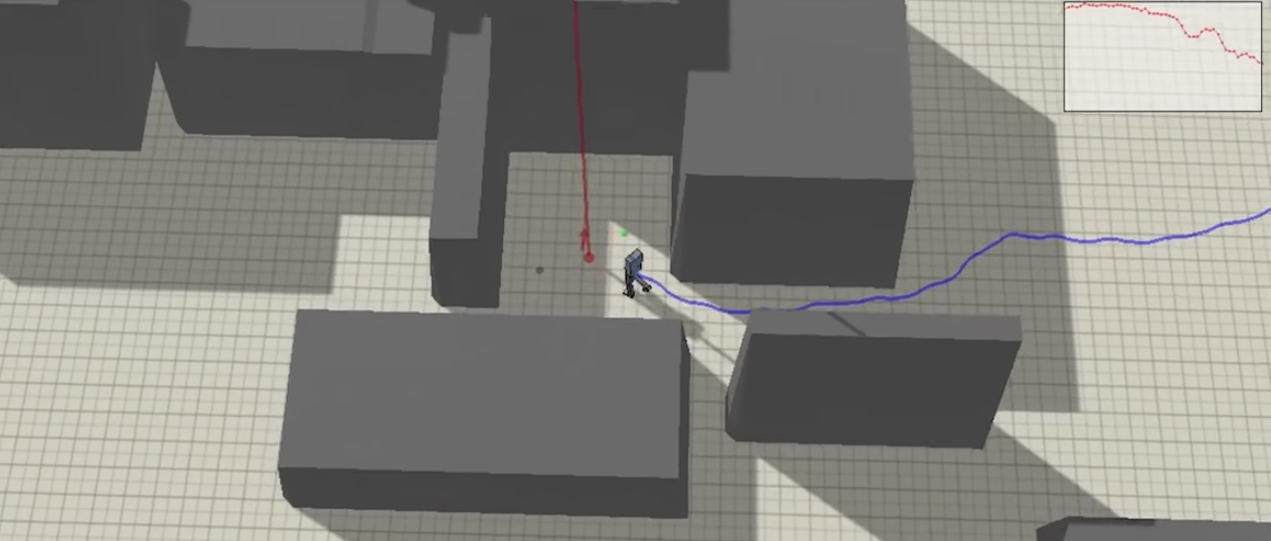
\includegraphics[width=1.0\textwidth]{./chapters/chapter_3/imgs/img_ch3_terrainrlsim_9.png}
            \caption{}
        \end{subfigure}

        \centering
        \begin{subfigure}[b]{0.3\textwidth}
            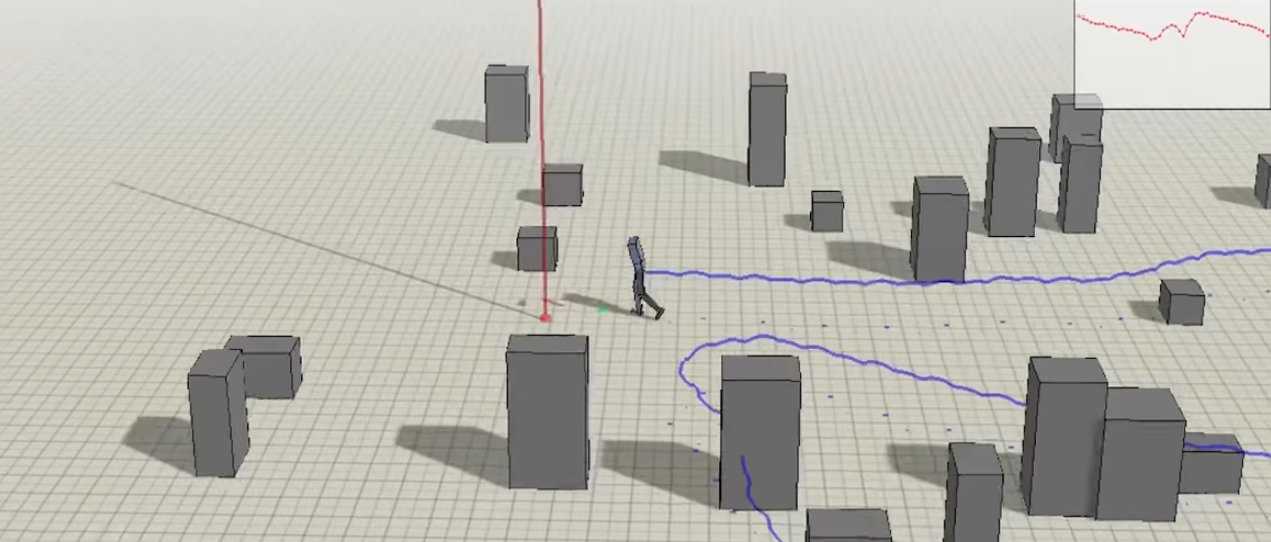
\includegraphics[width=1.0\textwidth]{./chapters/chapter_3/imgs/img_ch3_terrainrlsim_10.png}
            \caption{}
        \end{subfigure}

        \caption{Some of the tasks provided by the TerrainRLSim benchmark.}
        \label{fig:ch3_terrainrlsim}
    \end{figure}
}

\newcommand{\figBenchmarksUnityMLAgents}{
    \begin{figure}[!ht]
        \centering
        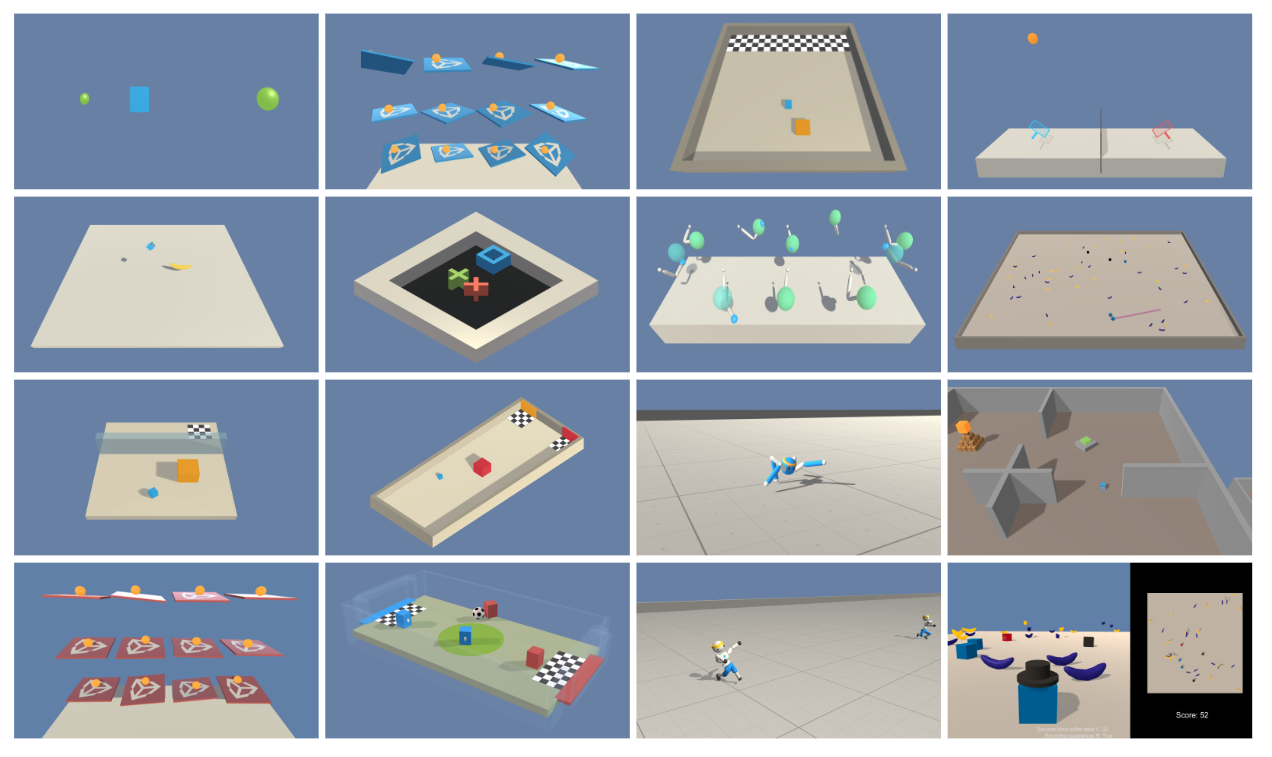
\includegraphics[width=1.0\textwidth]{./chapters/chapter_3/imgs/img_ch3_unity_ml_agents.png}
        \caption{Tasks available in the Unity ML-Agents framework.}
        \label{fig:ch3_unity_ml_agents}
    \end{figure}
}

\newcommand{\figBenchmarksMarathonEnvs}{
    \begin{figure}[!ht]
        \centering
        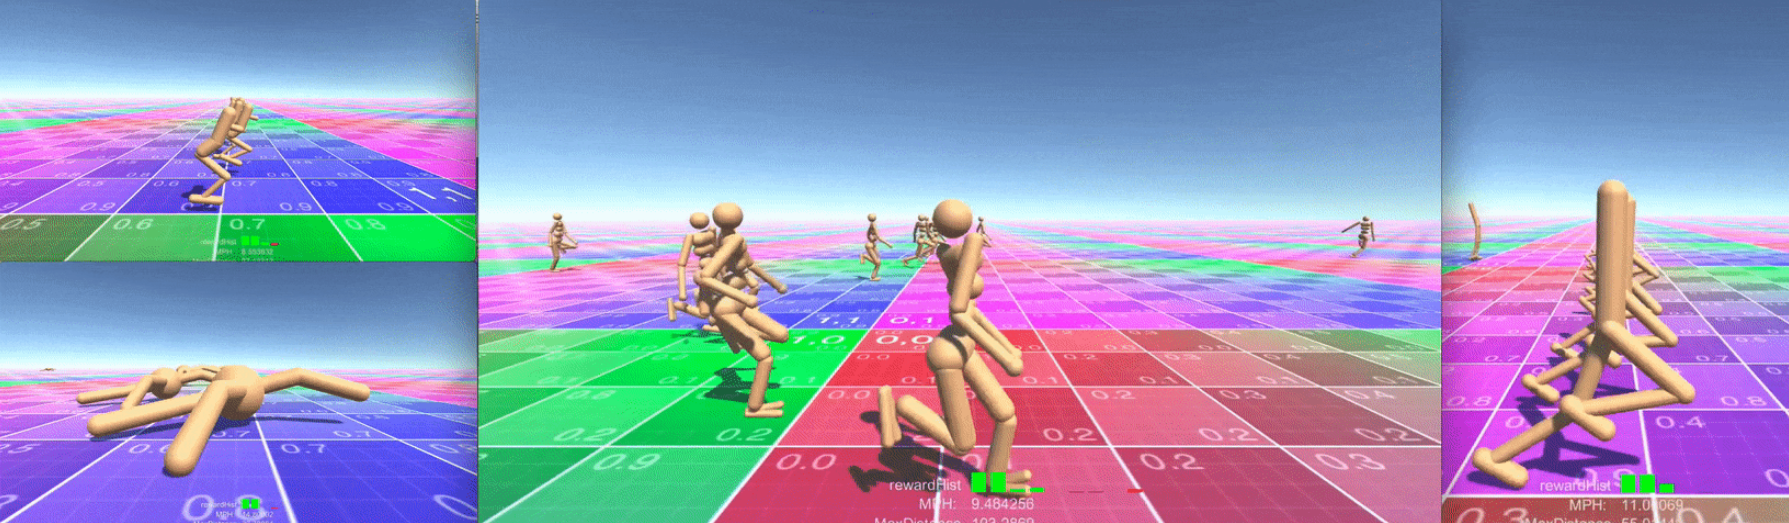
\includegraphics[width=1.0\textwidth]{./chapters/chapter_3/imgs/img_ch3_marathon_envs.png}
        \caption{Tasks available in the Marathon benchmark, provided along with the Unity ML-Agents framework.}
        \label{fig:ch3_marathon_envs}
    \end{figure}
}
%%%%%%%%%%%%%%%%%%%%%%%%%%%%%%%
%   Algorithms for chapter 3
%%%%%%%%%%%%%%%%%%%%%%%%%%%%%%%

\todo{En la sección 3.1 hay muchas definiciones y algoritmos, parece que debería estar en la sección de background, es la impresión que queda. Tal vez mejora si se presenta como la sección 3.2. En fin, lo podemos dejar así y ver que opina el jurado.}

In this chapter we will give an overview of current state of the art DeepRL algorithms
used in locomotion tasks, which will be the baselines we will evaluate with the proposed
framework. We also discuss various recent works in locomotion which also apply 
these algorithms. Finally we give an overview of the current benchmarks being
used for locomotion tasks.

\section{Deep RL algorithms for locomotion} \label{sec:ch3_deeprl_algorithms}

Current state of the art DeepRL algorithms used in locomotion tasks are \textbf{Policy Based} 
algorithms (or variants), which were introduced in section ~\ref{subsec:ch2_policyBasedMethods}. 
These variants address various problems with the standard Vanilla Policy Gradient algorithm,
which include:

\begin{itemize}
    \item \textbf{Step size selection}: The step size is of major importance in DeepRL,
          because the data the agent gets, which is then used for learning, is obtained
          using the policy, which is changed every gradient update step. Besides, the advantage
          signal that we estimate is very noisy, and this can lead to bad updates.

    \item \textbf{Sample efficiency}: The vanilla version of policy gradients uses
          the sampled data for only a single gradient estimation and update. This is
          very inefficient because the data sampled from the environment usually involves
          running the simulation for various episodes, which in some cases is very 
          computationally expensive.
\end{itemize}

To address these issues one approach is to turn the RL problem into a small 
optimization problem for each policy update. One simple way to achieve this
result is to use the loss function from ~\ref{eq:ch2_vpg_loss}, which allows to
reuse the collected data as much as possible until convergence. This results
in the following small optimization problem.

\begin{equation}
    \theta_{new} = \arg \max_{\theta} \mathbb{\hat E}_{t} 
                        \left [
                            \log \pi_{\theta}(a_{t}|s_{t}) \hat A_{t}
                        \right ]
\end{equation}

Unfortunately we cannot use this update until convergence, because of the issues
mentioned before. To avoid updating the policy too much we place a constraint in
the optimization problem by forcing small changes in the policy parameters. We also
makes a change in the loss function, and instead of using the simpler loss $L^{PG}$
we use a loss $L^{IS}$, which is derived using importance sampling (both result in
the same gradient). This results in the following constrained optimization problem.

\begin{align}
    \theta_{new} = \arg \max_{\theta} \mathbb{\hat E}_{t} 
                        \left [
                            \frac{\pi_{\theta}(a_{t}|s_{t})}
                                 {\pi_{\theta_{old}}(a_{t}|s_{t})} \hat A_{t}
                        \right ] \nonumber \\
    \textit{subject to: } 
                \Vert \theta - \theta_{old} \Vert_{2} \leq \delta
\end{align}

Even though we have a constrained the optimization problem with a threshold in the
Euclidean \todo{Nombres propios en Mayúsculas Euclidean} distance of the policy parameters, this usually does not yield the desired
results. For example, suppose we have a stochastic policy over a discrete action
space of two actions, parameterized using a single parameter  $\theta$ and a sigmoid 
function $\sigma$ in the following form.

\begin{gather*}
    \pi_{\theta}(a) = 
            \begin{cases}
                \sigma(\theta)          & a = 1 \\
                1 - \sigma({\theta})    & a = 2
            \end{cases}
\end{gather*}

Two fixed changes in the policy parameter $\theta$ give very different changes in
the output probabilities of the policy. The following figure shows this issue for
the case of $\Delta \theta=2$, applied in $\theta=$ 0, 2 and 4.

\figPolicyChanges

\subsection{Natural Policy Gradients}

A better policy update was proposed by \cite{NaturalPolicyGradient}, in which
the author \todo{sólo es un autor} proposed using the natural gradient instead of the a simple gradient 
update.

\begin{equation}
    \tilde{\nabla}_{\theta} J(\theta) = F^{-1}(\theta) \nabla_{\theta} J(\theta)
\end{equation}

This update makes use of the \textit{Fisher Information Matrix} $F$, which is used
to compensate the effects mentioned previously. This update also arises by reformulating
the small optimization problem into the following form:

\begin{align} \label{eq:}
    \theta_{new} = \arg \max_{\theta} \mathbb{\hat E}_{t} 
                        \left [
                            \frac{\pi_{\theta}(a_{t}|s_{t})}
                                 {\pi_{\theta_{old}}(a_{t}|s_{t})} \hat A_{t}
                        \right ] \nonumber \\
    \textit{subject to: } 
                \bar{D}_{KL}(\theta||\theta_{old}) \leq \delta
\end{align}

The only difference is the change of the euclidean constraint in parameter space
to the constraint in the KL-divergence of the parameterized probability distributions,
which ensures that the changes in parameter space made do not change the resulting 
distribution over action drastically. By solving this optimization problem using
linearization (Taylor Expansions) we obtain the following algorithm.

\algNaturalPolicyGradients

\subsection{Trust Region Policy Optimization (TRPO)}

The previous algorithm requires the inversion of the Fisher information matrix, which
is costly depending on the size of the parameters space (how big is the function approximator).
Also, it does not give theoretical improvement guarantees about the results, although
it provided better updates than the Vanilla Policy Gradient. \cite{TRPO} introduced
important changes that allow to solve the inversion issue, and also provided theoretical 
improvement guarantees on the policy updates (each update is guaranteed to improve performance).
The changes they introduced are listed below, and the resulting algorithm is shown in
Algorithm ~\ref{alg:trpo}.

\begin{itemize}
    \item Use the \textbf{conjugate gradient method} to avoid computing the inverse.
    \item Perform \textbf{line search} in the step size to make the largest update
          that satisfies the KL constraint.
\end{itemize}

\algTRPO

Some results (from the authors) of this algorithm in locomotion tasks and video game playing tasks 
can be found in the following \href{https://youtu.be/jeid0wIrSn4}{link}.

\subsection{Proximal Policy Optimization (PPO)}

This algorithm was introduced by \cite{PPO}, and it also tries to make the biggest
update possible while satisfying the same constraints and using all the data collected
for that optimization step. The authors proposed a simpler algorithm that requires
only an optimization over a surrogate loss function that approximates the behaviour
of the KL constraint. This loss in shown in the following equation. 

\begin{equation}
    L^{CLIP}(\theta) = \min \left ( \frac{\pi_{\theta}(a|s)}{\pi_{\theta_{old}}(a|s)} A^{\pi_{old}},
                                clip \left ( 
                                \frac{\pi_{\theta}(a|s)}{\pi_{\theta_{old}}(a|s)},
                                1-\epsilon, 1+\epsilon
                                     \right ) A^{\pi_{old}} \right )
\end{equation}

By using this loss in the optimization problem the resulting algorithm solves a similar
objective to TRPO, but without formulating the constrained optimization problem nor
using second order optimization, which is slightly costly in the TRPO implementations.
The resulting algorithm is shown below.

\algPPO

Some results (from the authors) of this algorithm in locomotion tasks and video game playing tasks 
can be found in the following \href{https://blog.openai.com/openai-baselines-ppo/}{link}.

\newpage

\section{DeepRL applied to locomotion}

In this section we discuss current state of the art results of DeepRL in locomotion 
tasks. These served as the inspiration for this proposal which serves in part as an 
extension of these results to more diverse and diverse environments.

\subsection{Benchmarking DeepRL for Continuous Control}

\cite{Rllab} presented a benchmark suite for continuous control tasks, which is
known as \textbf{Rllab} (discussed in section ~\ref{subsec:ch3_rllab}). They 
introduced this benchmark along with some baselines that consisted of implementations of 
various state of the art algorithms in that time, like Trust Region Policy Optimization 
(\citeauthor{TRPO}), Truncated Natural Policy Gradients (\citeauthor{NaturalPolicyGradient}, 
\citeauthor{TNPG1}, \citeauthor{TNPG2}), and Deep Deterministic Policy Gradients \citep{DDPG}, 
as well as some base algorithms like Vanilla Policy Gradients (\citeauthor{REINFORCE}, 
\citeauthor{PGSutton}), and some derivate-free algorithms like Cross-Entropy methods 
(\citeauthor{CrossEntropyMethods}, \citeauthor{CrossEntropyTetris}).

Our proposal is similar to this work, in the sense that we propose a new set of
benchmarks and a set of corresponding baselines tested in this new environments.
A key difference is that this benchmark consists of simple environments, mostly
in flat terrain, although they also proposed some other environments that have a
more hierarchical structure, and some that have partial observability. For more
details of the benchmark itself, please refer to section ~\ref{subsec:ch3_rllab}.

\subsection{DeepTerrainRL}

\cite{DeepTerrainRL} presented very promising results for locomotion of simulated
characters. Their agents were able to traverse complex terrain using very natural
behaviours (see Figure ~\ref{fig:ch3_deepterrainrl}). Some footage of their results
can be found in \href{https://xbpeng.github.io/projects/DeepTerrainRL/}{this} link.
Some key aspects of this work consist of:

\figDeepTerrainRL
\figDeepTerrainRLcharacterFeatures
\figDeepTerrainRLMACE

\begin{itemize}
    \item \textbf{High dimensional features}: the authors used a high dimensional 
          state representation as the input to the policies of the agent.
          This is different from previous work were they relied on hand crafted
          features engineered to complete the specific task. These features (shown in
          Figure ~\ref{fig:ch3_deepterrainrl_state_features}) consisted on character 
          features (links positions and velocities), and terrain features (1D heightfield 
          of the terrain ahead).


    \item \textbf{Usage of multiple actor policies}: the authors used an approach
          called Mixture of Actors and Critics Experts, in which the use various
          actor policies that are used in specific situations, given by the decisions 
          of the critics. This approach is shown in Figure ~\ref{fig:ch3_deepterrainrl_mace},
          and it is shown in action in Figure ~\ref{fig:ch3_deepterrainrl}, where the
          color of the trail that the agent leaves corresponds to the choice of actor
          used for that specific situation.

          The computed actions for the chosen actors are then sent to a Finite State
          Machine controller, which has 29 input parameters consisting of leg forces,
          PD joint targets, and PD velocity feedback gains.

    \item \textbf{Complex terrain}: the approach presented by the authors
          worked in their proposed environments, which consisted in complex terrain
          generated along a fixed direction. The authors developed a simulator on
          top of Bullet, which allowed them to create complex tasks that were then
          used in future research (\cite{ActuationChoice}, \cite{DeepLoco}, \cite{DeepMimic})
          and would be later open sourced into a package called TerrainRLSim \citep{TerrainRLSim}.

    \item \textbf{Initialization}: the resulting policies \textbf{are not learned from scratch}.
          The authors used an initialization procedure to obtain a set of working
          behaviours (walking, jumping) that served as the basis for the training
          of the agents. The policies are also very structured (using a FSM controller),
          and although giving good results this structure is hand engineered. Some
          example of the initialization can be found \href{https://youtu.be/8qQmL3f2fd8?t=587}{here}.

    \item \textbf{Network architecture}: the actors and critics for each
          agent were parameterized using deep neural networks, which processed the
          high dimensional state representation and output the corresponding results
          for the actors and critics (see Figure ~\ref{fig:ch3_deepterrainrl_architecture}).
          The terrain features are processed using convolutional layers, and then
          the resulting features are concatenated to the character features. These
          feature vectors are then used by fully connected layers that branch out
          to each actor and critic. Note that the actors and critics share weights
          up until the concatenation step of character and extracted terrain feature vectors.

          \figDeepTerrainRLArchitecture

    \item \textbf{Learning algorithms}: for training the authors used the CACLA 
          algorithm, developed by \cite{CACLA}.

\end{itemize}

\subsection{DeepLoco}

\cite{DeepLoco} consisted of a follow up work from the one we discussed previously.
This work presented a hierarchical system that successfully learned locomotion skills
for more complicated tasks (compared to forward terrain traversal). Some of the tasks
that the agent successfully completed are shown in Figure ~\ref{fig:ch3_deeploco_tasks},
and a video from their results can be found \href{https://youtu.be/hd1yvLWm6oA}{here}

\figDeepLocoTasks

Some key aspects of this work are the following:

\begin{itemize}
    \item \textbf{A hierarchical system}: the approach proposed was to use a two-level
          hierarchical controller (Figure ~\ref{fig:ch3_deeploco_system}), which consisted 
          of a high-level controller that gave a heading direction and foot placement 
          positions, and a low-level controller that generated the appropriate gait 
          to satisfy this command.

          \figDeepLocoSystem

    \item \textbf{High dimensional features}: similar to the previous work, the state
          representation used is high dimensional (see Figure ~\ref{fig:ch3_deeploco_state_features}), 
          with a 2D heightmap replacing the previous 1D choice.

          \figDeepLocoStateFeatures

    \item \textbf{Structure of the controller}: the methods used impose some structure
          into the controller and the whole process. The approach is again not learn
          the skills from scratch, compared to the results of a related work by
          \cite{HeessLearningAndTransfer} (see some results in \href{https://youtu.be/sboPYvhpraQ?t=34}{this} video), 
          in which the skills are learned without reference motions and extra pre processing
          steps for initial learning (although they also do some initialization steps
          for learning low-level skills).

    \item \textbf{Complex tasks}: finally, the tasks presented in this work were
          much more complex (see Figure ~\ref{fig:ch3_deeploco_tasks}), and required
          more hierarchical reasoning. As shown in the first presented work related evaluation
          of DeepRL algorithms \citep{Rllab}, some simple tasks required hierarchical
          reasoning, and single low-level policies were not able to complete these tasks.

    \item \textbf{Learning algorithms}: the learning algorithm is the same used in
          their previous work (CACLA, by \citeauthor{CACLA}).

\end{itemize}

\subsection{Emergence of Locomotion}

The authors of \cite{DeepmindEmergenceLocomotion} studied the same problem of locomotion
as in \cite{DeepTerrainRL}. They developed an agent that could traverse obstacles
courses that consisted of terrain generated \textbf{procedurally} in a single forward
direction, shown in Figure ~\ref{fig:ch3_emergence_of_locomotion_tasks}. Their results
can be seen in action in \href{https://youtu.be/hx_bgoTF7bs}{this} video.

\figEmergenceOfLocomotionTasks

Some key aspects of this work are the following:

\begin{itemize}
    \item \textbf{High dimensional state representation}: the authors used a similar
          state representation to the previously discussed works, which is shown in
          Figure ~\ref{fig:ch3_emergence_of_locomotion_state_representation}.

          \figEmergenceOfLocomotionStateRepresentation

    \item \textbf{Complex terrain and curricula usage}: the authors also used more complicated
          terrain (compared to flat terrain benchmarks) using procedural terrain 
          generation (see Figure ~\ref{fig:ch3_emergence_of_locomotion_terrains}). 
          They also added a curriculum to the terrain creation procedure, which allow them 
          to increase progressively the difficulty of the terrain generated.

          \figEmergenceOfLocomotionTerrain

    \item \textbf{Learning from scratch}: one of the key features of this work is
          that the skills acquired are learned from scratch without previous initialization
          nor motion reference, compared to the related works discussed previously.
          However, because no reference is given the resulting policies give locomotion 
          behaviours that are idiosincratic, and in some cases even humorous (see
          \href{https://youtu.be/hx_bgoTF7bs?t=87}{this} video for a reference of an 
          humanoid with a peculiar gait). Also, the learning algorithm used is a distributed
          variant of the PPO algorithm \citep{PPO}.

    \item \textbf{Learning algorithms}: the authors used a distributed version
          of the PPO \citep{PPO} algorithm for their main results, but they also 
          tested some other algorithms, like TRPO \citep{TRPO} and A3C \citep{A3C}, 
          in order to make comparisons.

\end{itemize}

%% \subsection{DeepMimic}
%% 
%% \newpage

\section{DeepRL locomotion benchmarks}

\subsection{Deepmind ControlSuite}

This set of benchmarks was first introduced in \cite{Controlsuite}, and consists 
of various locomotion tasks (shown in Figure ~\ref{fig:ch3_controlsuite}), with various types of agents 
to select from. The models available consist of xml files in the mujoco format (mjcf) 
that are used as the blueprints to instantiate an agent. The tasks consist of the specific
setups that the agents must solve, like walking, standing, running, etc.

\figBenchmarkControlSuite

As described in their \href{https://arxiv.org/pdf/1801.00690.pdf}{technical report}\todo{Tal vez colocar un footnote porque no será posible ver la referencia al imprimir el documento, verificar otras referencias similares en otras partes de la tesis},
some of the key features of this benchmark include:

\begin{itemize}
    \item \textbf{Full state observations}: the observations provided to the agent
          are sufficient to recover the full state of the environment. These observations
          include positions and velocities (of bodies and joints), touch sensor readings,
          and some other task specific measurements. Using this information, the full state
          of the environment can be recovered due to the simple nature of the environment 
          (most locomotion tasks in the benchmark are flat terrain tasks, and no information
          is hidden from the agents).

    \item \textbf{Normalized actions}: the actions exposed to the user have been normalized 
          in the range $\left[-1,1\right]$. These are mapped to actuators that represent
          torques applied to joints (torque actuation model).

    \item \textbf{Normalized rewards}: the rewards are set to the range $\left[ 0, 1 \right]$, 
          and can be smooth (whole range) or sparse (just the values $\left\{0,1\right\}$).

    \item \textbf{MuJoCo backend}: MuJoCo is the underlying physics backend, and it is
          integrated into the suite by using Python bindings generated using 
          \href{https://github.com/deepmind/dm_control/blob/master/dm_control/autowrap/autowrap.py}{ctypes}.
\end{itemize}

\subsection{OpenAI Gym}

This set of benchmarks consists of two separate options depending on the physics 
backend (MuJoCo and Bullet). These two options are Python Wrappers for the supported 
physics backends and are used as low level functionality for the high level API provided by Gym \citep{Gym}.
The options used as wrappers for the two physics backends available are the following:

\begin{itemize}
    \item \textbf{Mujoco-py} : A Python wrapper for MuJoCo, very similar to ControlSuite. 
          The available tasks are similar to the ones in ControlSuite, which are shown 
          in Figure ~\ref{fig:ch3_openaigym_mujoco}.

        \figBenchmarkOpenAIGymMujoco

    \item \textbf{RoboSchool}: An implementation that uses PyBullet, which exposes 
          the Bullet physics engine through a Python API. The environments exposed 
          are a bit different to the previous suite, and are shown in Figure ~\ref{fig:ch3_openaigym_roboschool}. 

        \figBenchmarkOpenAIGymRoboschool

\end{itemize}

The RL API exposed by Gym is similar to the one exposed by ControlSuite. 
In each step taken in the environment, the API returns the observation, 
reward, and some extra observations. More information can be found in its 
technical report \citep{Gym}, and in its \href{https://github.com/openai/gym}{repository}.

\subsection{Rllab and Garage} \label{subsec:ch3_rllab}

Rllab is a set of benchmarks similar to the previous two. It implements its own 
Python wrapper for MuJoCo, and builds its own Reinforcement Learning API on top 
of that wrapper. It provides a set of tested baselines of various Deep Reinforcement 
Learning algorithms, which were presented in \cite{Rllab}. The environments provided 
by Rllab are grouped in three categories: \textbf{classic} (Figure ~\ref{fig:ch3_rllab_classic}), 
\textbf{locomotion} (Figure ~\ref{fig:ch3_rllab_locomotion}) and \textbf{hierarchical} 
(Figure ~\ref{fig:ch3_rllab_hierarchical}). It is compatible with Gym, by means of 
a wrapper on top of its environments, but as they explain in their documentation 
\href{https://rllab.readthedocs.io/en/latest/user/gym_integration.html}{website} 
this is a very different API.

\figBenchmarkRllabClassic

\figBenchmarkRllabLocomotion

\figBenchmarkRllabHierarchical

Garage is the next version of the Rllab suite, and is very similar in architecture 
to Rllab, with support for more environments and baselines. To this date the number 
of environments is similar to the ones in Rllab, but is being actively supported, 
compared to Rllab. More information can be found in its \href{https://github.com/rlworkgroup/garage}{repo}.

\subsection{Robosuite}
 
\href{https://github.com/StanfordVL/robosuite/}{Robosuite} is a set of benchmarks first 
introduced along the \href{https://surreal.stanford.edu/}{Surreal} 
framework by \cite{Surreal}. This set of benchmarks is more oriented towards robot manipulation,
providing tasks that involve robot models commonly used as robotics manipulation research platforms 
(like \textit{sawyer} and \textit{baxter}).

This set of benchmarks use MuJoCo as physics backend (through mujoco-py), and as they
explain in their documentation, the suite provides various APIs that allow the user
to create diverse experiments. By using its programmatical task construction API
the user can create an specific setup with just a few lines of Python code.
The tasks provided in the suite are shown in Figure ~\ref{fig:ch3_robosuite}.

\figBenchmarksRobosuite

\subsection{Gpu-Accelerated Simulation}

This set of benchmarks was presented in \cite{GpuSim}, and makes use of a custom 
physics backend developed in-house. The physics simulator is built on top of the 
NVIDIA FleX physics engine, which focuses on accelerated GPU physics simulation. 
This approach allows to run scenes with a large number of agents, ranging in the 
thousands. One key detail to consider is the usage of FleX, which is a position 
based dynamics engine. This type of simulations allows for fast simulation by trading
accuracy. 

The simulator is not yet released (as stated by the authors, it is still 
work in progress), but will probably be released as part of the 
\href{https://developer.nvidia.com/isaac-sdk}{NVIDIA Isaac platform}. Some of the 
benchmarks presented are shown in Figure ~\ref{fig:ch3_gpusim}, and include tasks
involving hundreds of humanoids running in environments from low to high complexity.

\figBenchmarksGpuSim

\subsection{TerrainRLSim}

This set of benchmarks was presented in \cite{TerrainRLSim}, and was used in \cite{DeepTerrainRL}, 
\cite{ActuationChoice} as the core framework. This suite uses Bullet as physics backend,
and one key difference with the other presented works is the diversity of the tasks provided.
The tasks provided are shown in Figure ~\ref{fig:ch3_terrainrlsim}, and range from 
single direction obstacle courses, to two dimensional traversal tasks.

\figBenchmarksTerrainRLSim

\subsection{Unity ML-Agents}

This set of benchmarks was presented in \cite{UnityMLAgents}, and it is a framework 
built on top the \citeauthor{Unity} game engine, which makes use of PhysX as backend. 
The tasks are ports of various tasks from the previous benchmarks, and can be used
through a Python API that connects to the games that represent the tasks. The base tasks
provided by the framework are shown in Figure ~\ref{fig:ch3_unity_ml_agents}. Also, 
there are a set of tasks that are provided on top of this framework through the 
\href{https://github.com/Unity-Technologies/marathon-envs}{Marathon Environments} 
package, and are shown in Figure ~\ref{fig:ch3_marathon_envs}.

\figBenchmarksUnityMLAgents

\figBenchmarksMarathonEnvs

\section{Summary}

In this chapter we presented various related works from which we take inspiration
for our proposal (presented in Chapter ~\ref{ch:intro}, and detailed in the next
chapter). Some key ideas from this chapter are shown below.

\begin{itemize}
    \item We presented current state-of-the-art algorithms used in locomotion, 
          namely TRPO \citep{TRPO} and PPO \citep{PPO}. These algorithms were
          based in the Vanilla Policy Gradients method (section ~\ref{subsec:ch2_policyBasedMethods}), 
          and try to solve problems like step size selection and sample efficiency.
          These algorithms are going to be implemented as baselines for our evaluations
          in the environments that we will implement as part of the framework.

    \item We also presented some success stories of DeepRL in locomotion, like
          \citet{Rllab}, \citet{DeepTerrainRL}, \citet{DeepLoco} and \citet{DeepmindEmergenceLocomotion}.
          We take inspiration from these works for various features of our framework:
          environments, tasks, state representation, etc..

    \item Finally, we presented currently available benchmarks for DeepRL in locomotion,
          and showed some details of their support and features that they provide. We
          emphasize the fact that most of these benchmarks do not provide diverse
          enough environments, which is a key aspect that our proposed framework
          tries to solve.
\end{itemize}

In the next chapter we will give more details about our proposal. We will discuss
some of the high level aspects of our proposal, as well as give more technical details
about the approach for its implementation.